% Behavior tree of The Thresher, Vagrancy (data/pilots.json, "thresher": a loop pilot,
% pattern "overhead", pause_ticks 90). Drawn in behavior-tree notation.
% Standalone: compiles on its own in Overleaf with pdflatex.
\documentclass[tikz,border=4pt]{standalone}
\usetikzlibrary{arrows.meta,shapes.geometric,positioning,calc}
\usepackage{amssymb}   % \rightrightarrows and \circlearrowright

% --- Colors: the deck's palette --------------------------------------------
\definecolor{paper}{HTML}{FDFDFC}   % node fill
\definecolor{ink}{HTML}{1B2430}     % text and edges
\definecolor{muted}{HTML}{6B7680}   % legend
\definecolor{cond}{HTML}{2F4BA0}    % condition leaves
\definecolor{act}{HTML}{2A6B4A}     % action leaves

% --- Layout, in centimetres --------------------------------------------------
\newcommand{\BoxW}{3.4cm}       % width of every leaf box
\newcommand{\StepGap}{4.0}      % horizontal distance between the swing's steps
\newcommand{\RootX}{8.4}        % the root's horizontal position
\newcommand{\RepeatY}{-2.2}     % height of the repeat decorator
\newcommand{\SeqY}{-4.0}        % height of the sequence nodes
\newcommand{\LeafY}{-6.2}       % height of the leaves
\newcommand{\WalkX}{14.8}       % horizontal position of the walking branch
\newcommand{\WalkGap}{200}      % distance (cm) beyond which it walks toward you

\begin{document}
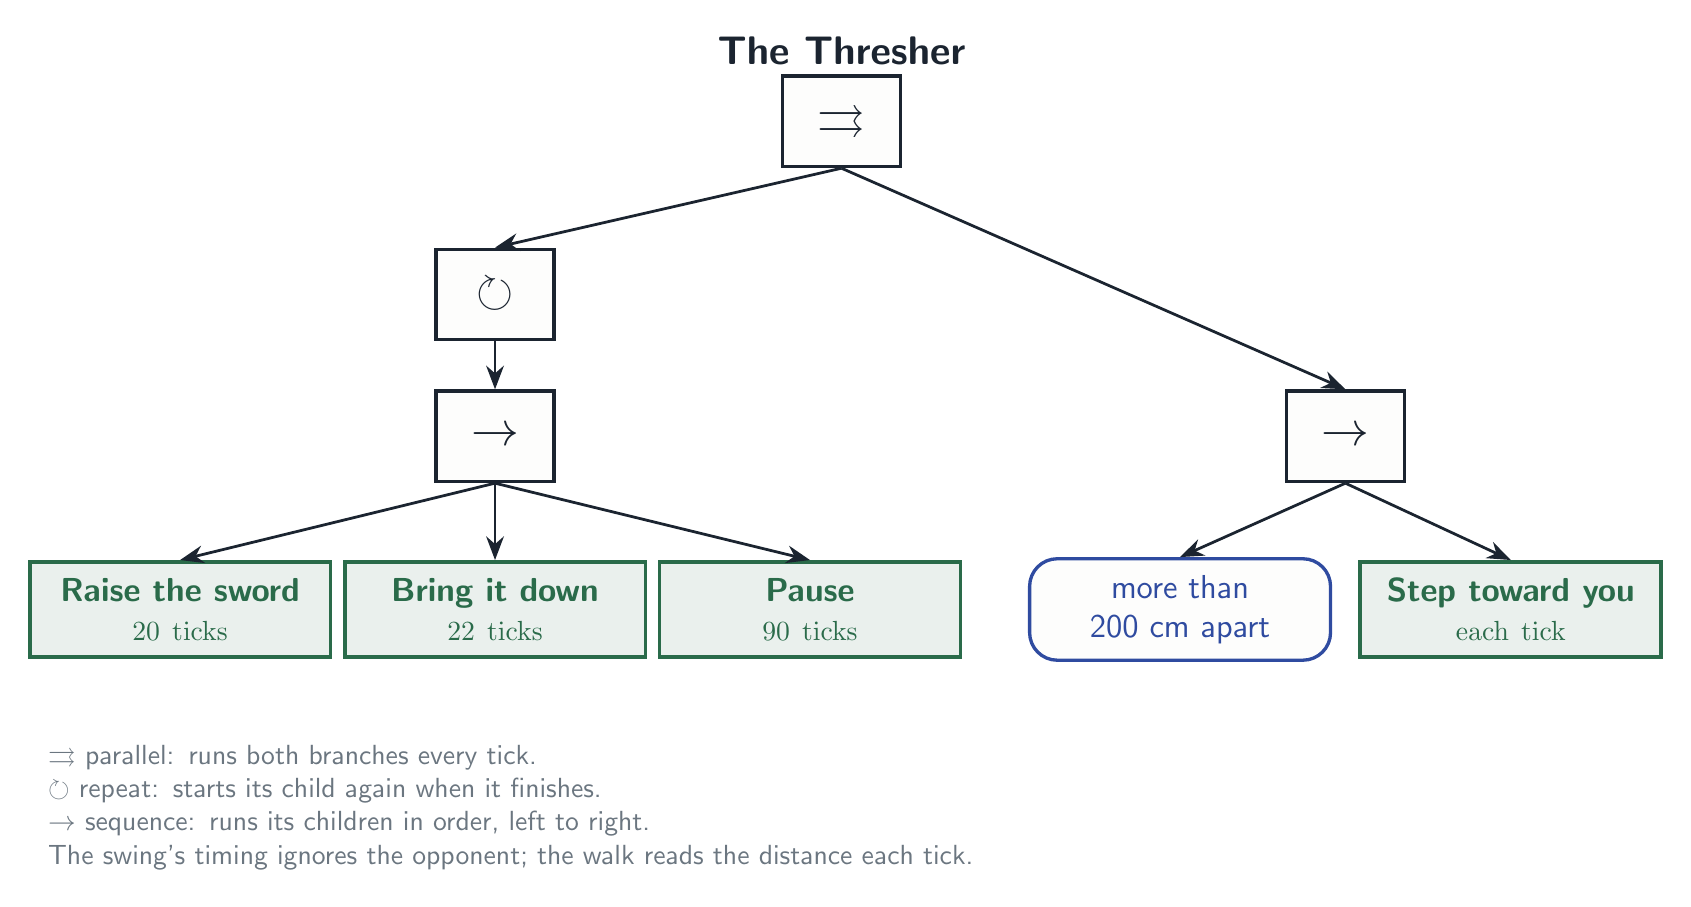
\begin{tikzpicture}[
    font=\sffamily\large, ink,
    edge/.style={-{Stealth[length=3mm]}, line width=1pt, draw=ink},
    control/.style={draw=ink, line width=1.2pt, fill=paper, minimum width=1.5cm, minimum height=1.15cm, font=\sffamily\bfseries\LARGE},
    condition/.style={draw=cond, line width=1.2pt, rounded corners=10pt, fill=paper, text width=\BoxW, align=center, inner sep=6pt, text=cond},
    action/.style={draw=act, line width=1.4pt, fill=act!10, text width=\BoxW, align=center, inner sep=6pt, text=act, font=\sffamily\large\bfseries},
  ]

% --- Root: run both branches every tick --------------------------------------
\node[control] (root) at (\RootX, 0) {$\rightrightarrows$};
\node[anchor=south, font=\sffamily\bfseries\Large] at (root.north) {The Thresher};

% --- The swing: a sequence, repeated forever ---------------------------------
\node[control] (repeat) at (\StepGap, \RepeatY) {$\circlearrowright$};
\node[control] (seq) at (\StepGap, \SeqY) {$\rightarrow$};
\foreach \i/\what/\ticks in {0/{Raise the sword}/20, 1/{Bring it down}/22, 2/{Pause}/90} {
  \node[action] (step\i) at (\i*\StepGap, \LeafY) {\what \\ {\normalfont\normalsize \ticks{} ticks}};
  \draw[edge] (seq.south) -- (step\i.north);
}

% --- The walk: a sequence checked every tick -----------------------------------
\node[control] (walk) at (\WalkX, \SeqY) {$\rightarrow$};
\node[condition] (far) at (\WalkX-2.1, \LeafY) {more than \WalkGap{} cm apart};
\node[action] (step) at (\WalkX+2.1, \LeafY) {Step toward you \\ {\normalfont\normalsize each tick}};
\draw[edge] (walk.south) -- (far.north);
\draw[edge] (walk.south) -- (step.north);

% --- Edges from the root and the decorator -------------------------------------
\draw[edge] (root.south) -- (repeat.north);
\draw[edge] (repeat.south) -- (seq.north);
\draw[edge] (root.south) -- (walk.north);

% --- Annotations ---------------------------------------------------------------
\node[anchor=north west, text=muted, font=\sffamily\normalsize, align=left, text width=17.5cm] at (-1.8, -7.8)
  {$\rightrightarrows$ parallel: runs both branches every tick.\\
   $\circlearrowright$ repeat: starts its child again when it finishes.\\
   $\rightarrow$ sequence: runs its children in order, left to right.\\
   The swing's timing ignores the opponent; the walk reads the distance each tick.};

\end{tikzpicture}
\end{document}

% --- Self-check ----------------------------------------------------------------
% Steps and lengths: the \foreach list is Looper::new's "overhead" pattern in
%   crates/pilot/src/lib.rs: SHOULDER_UP 20, SHOULDER_DOWN 22, then pause_ticks (90).
% Repetition: the pattern index wraps to the start (at + 1 mod len): the repeat node.
% Walking: Looper::input steps toward the opponent when drift is false and gap > 200,
%   every tick and alongside the swing: the parallel root and \WalkGap.
